\documentclass{article}

% if you need to pass options to natbib, use, e.g.:
% \PassOptionsToPackage{numbers, compress}{natbib}
% before loading nips_2016
%
% to avoid loading the natbib package, add option nonatbib:
% \usepackage[nonatbib]{nips_2016}

\usepackage{nips_2016}

% to compile a camera-ready version, add the [final] option, e.g.:
% \usepackage[final]{nips_2016}

\usepackage[utf8]{inputenc} % allow utf-8 input
\usepackage[T1]{fontenc}    % use 8-bit T1 fonts
\usepackage{hyperref}       % hyperlinks
\usepackage{url}            % simple URL typesetting
\usepackage{booktabs}       % professional-quality tables
\usepackage{amsfonts}       % blackboard math symbols
\usepackage{nicefrac}       % compact symbols for 1/2, etc.
\usepackage{microtype}      % microtypography
\usepackage{graphicx}

\title{Question Answering on Wikipedia using Memory Networks}

% The \author macro works with any number of authors. There are two
% commands used to separate the names and addresses of multiple
% authors: \And and \AND.
%
% Using \And between authors leaves it to LaTeX to determine where to
% break the lines. Using \AND forces a line break at that point. So,
% if LaTeX puts 3 of 4 authors names on the first line, and the last
% on the second line, try using \AND instead of \And before the third
% author name.

\author{
  Ashwin asokan
  \thanks{Use footnote for providing further
    information about author (webpage, alternative
    address)---\emph{not} for acknowledging funding agencies.} \\
  Department of Computer Science\\
  University of colorado Boulder\\
  \texttt{ashwin.asokan@colorado.edu} \\
  %% examples of more authors
  %% \And
  %% Coauthor \\
  %% Affiliation \\
  %% Address \\
  %% \texttt{email} \\
  %% \AND
  %% Coauthor \\
  %% Affiliation \\
  %% Address \\
  %% \texttt{email} \\
  %% \And
  %% Coauthor \\
  %% Affiliation \\
  %% Address \\
  %% \texttt{email} \\
  %% \And
  %% Coauthor \\
  %% Affiliation \\
  %% Address \\
  %% \texttt{email} \\
}

\begin{document}
% \nipsfinalcopy is no longer used

\maketitle

\begin{abstract}
  In this project, we investigate the task of building a Question Answering system using deep neural networks augmented with a memory component. Our goal is
to implement memory based neural network models, MemN2N and its extensions described in Sukhbaatar et al. (2015)[4], Attentive Reader described by Hermann et al.(2015) [5] and apply
it on the wiki-reading QA tasks introduced by Hewlett et al.(2016) [1]. Both the above models have the distinction of being weakly supervised and trained end to end, making it viable for realistic settings. They seem to show promising performance on synthetic question answering datasets and other language task like language modeling. We realize that unlike simulated datasets like bAbI,the memory models are not sufficient to achieve satisfactory performance on real-world QA datasets like Wiki QA. We leverage the works of these authors and explore few extensions to the proposed systems to make it work on these large datasets.
\end{abstract}

\section{Introduction}

Two interesting chanllenges in natural language processing research have been to build models capable of multiple computational steps to achieve a task and models that could describe long term dependencies in sequential data. The task of question answering (QA) aptly fits the former. Additionally, QA is extremely broad as many NLP tasks can be reformulated in the QA setup. This implies that devising better models for improving QA can be quite useful in different directions.

Fundamentally, QA systems need to perform two tasks: retrieval and inference. The QA system need to store the knowledge available in some convenient internal representation and subsequently search through the representation to find relevant bits to answer the question. Analyzing the knowledge to derive the required answer requires some form of inference.

In this work we investigate a particular class of learning models called memory networks. Memory networks consists of an inference component combined with a long term memory component. The memory component can be read, written to with the goal of predicting the best possible answer. We use large scale QA task as our benchmark to evaluate the effectiveness of these models. 

\section{Background}

\subsection{Memory Networks}

A memory network consists of a memory m(an array of objects indexed by $m_i$) and four (potentially learned) components I,G,O and R as follows:

I:  (input feature map) – converts the incoming input to the internal feature representation

G:  (generalization) – updates old memories given the new input.  We call this generalization as there is an opportunity for the network to compress and generalize its memories at this stage for some intended future use.

O: (output feature map) – produces a new output (in the feature representation space), given the new input and the current memory state.

R:  (response) – converts the output into the response format desired.  For example, a textual response or an action.

Given an input x (e.g., an input character, word or sentence depending on the granularity chosen, an
image or an audio signal) the flow of the model is as follows:

\begin{enumerate}
  \item Convert x to an internal feature representation I(x). 
  \item Update memories $m_i$ given the new input:
$ m_i = G(m_i, I(x),m), \forall i.$
  \item Compute output features o given the new input and the memory: $ o = O( I(x),m)$
  \item Finally, decode output features o to give the final response: r = R(o)
\end{enumerate}

I component: Component I can make use of standard pre-processing, e.g., parsing, coreference and entity resolution for text inputs. It could also encode the input into an internal feature representation, e.g., convert from text to a sparse or dense feature vector.

G component: The simplest form of G is to store I(x) in a “slot” in the memory:
\begin{equation}
m_{H(x)} = I(x)
\end{equation}
where H(.) is a function selecting the slot.  That is, G updates the index H(x) of m, but all other
parts of the memory remain untouched. More sophisticated variants of G could go back and update earlier stored memories (potentially, all memories) based on the new evidence from the current input x. If the input is at the character or word level one could group inputs (i.e., by segmenting them into chunks) and store each chunk in a memory slot.

If the memory becomes full,  a procedure for “forgetting” could also be implemented by H as it
chooses which memory is replaced, e.g.,H could score the utility of each memory, and overwrite the least useful. We have not explored this experimentally yet.

O and R components: The O component is typically responsible for reading from memory and performing inference, e.g., calculating what are the relev
ant memories to perform a good response. The R component then produces the final response given O.  For example in a question answering setup O finds relevant memories, and then R produces the actual wording of the answer, e.g., R could be an RNN that is conditioned on the output of O.

We investigate particular instantiation of memory networks where the components are neural networks. We refer to these as memory neural networks (MemNNs) and Attentive Reader neural networks (ARNNs). 

\subsection{Memory Neural Networks(MemNNs)}

Our model takes a discrete set of inputs $x_1,...,x_n$ that are to be stored in the memory, a query q, and outputs an answer a.  Each of the $x_i$,q, and a contains symbols coming from a dictionary with V words. The model writes all x
to the memory up to a fixed buffer size, and then finds a continuous representation for the x and q. The continuous representation is then processed via multiple hops to output a. This allows backpropagation of the error signal through multiple memory accesses back to the input during training.

Input memory representation: Suppose we are given an input set $x_1,..,x_i$ to be stored in memory. The  entire  set  of $x_i$ are  converted  into  memory  vectors $m_i$ of  dimension d computed  by embedding each $ x_i $ in a continuous space, in the simplest case, using an embedding matrix A(d,V). The query q is also embedded (again, in the simplest case via another embedding matrix B
with the same dimensions as A) to obtain an internal state u. In the embedding space, we compute the match between u and each memory $ m_i $ by taking the inner product followed by a softmax:
\begin{equation}
p_i = Softmax(u^T m_i)
\end{equation}

where $ Softmax(z_i) = e^{z_i} / \sum_j e^{z_j} $. Defined in this way p is a probability vector over the inputs.

Output  memory  representation: Each $x_i$ has  a  corresponding  output  vector
$c_i$ (given  in  the simplest case by another embedding matrix C). The response vector from the memory o is then a sum over the transformed inputs $c_i$, weighted by the probability vector from the input:
\begin{equation}
o = \sum_i p_i * c_i
\end{equation}
Because the function from input to output is smooth, we can easily compute gradients and backpropagate through it.

Generating the final prediction: In the single layer case, the sum of the output vector o and the input embedding u is then passed through a final weight matrix W(V,d) and a softmax to produce the predicted label:

\begin{equation}
\hat{a} = Softmax(W (o + u))
\end{equation}

During training, all three embedding matrices A,B and C, as well as W are jointly learned by minimizing a standard cross-entropy loss between $\hat{a}$ and the true label a. Training is performed using stochastic gradient descent.

\begin{figure}
  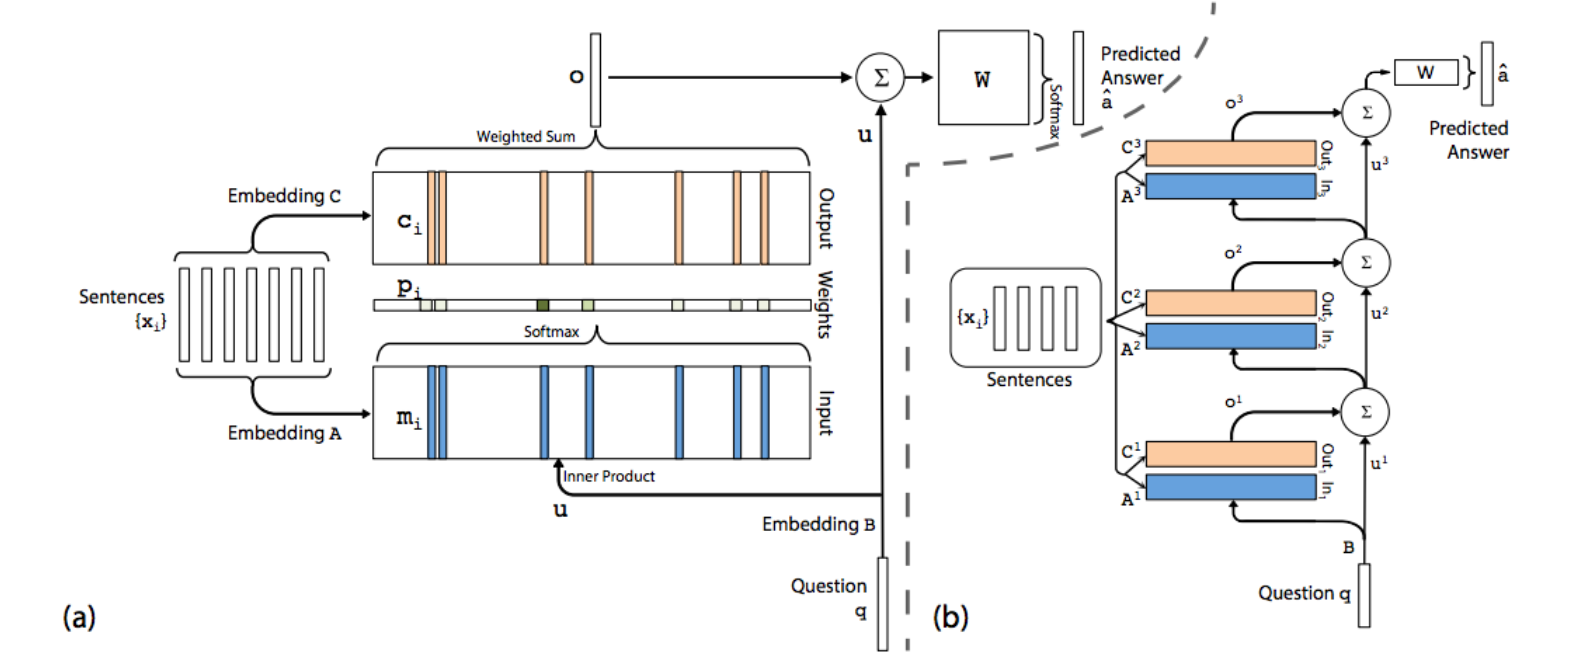
\includegraphics[width=\linewidth]{memory.png}
  \caption{ (a): Single layer version. (b): Three layer version }
  \label{fig:memory}
\end{figure}

\subsection{Attentive Reader(ARNNs)}

The naive LSTM Reader must propagate dependencies over long distances in order to connect queries to their answers.The fixed width hidden vector forms a bottleneck for this information flow that the attentive reader circumvents using an attention mechanism.This attention model first encodes the document and the query using separate bidirectional single layer LSTMs.

The first step of the model is to apply an encoding
to the context $ c = {c_1 , c_2 , ..., c_n }$ through a birectional LSTM network. The resulting forward and output vectors $ \overrightarrow{H_c} =\overrightarrow{(h_c)_i}$ and $ \overleftarrow{H_c} = \overleftarrow{(h_c)_i} $ are concatenated into a final paragraph representation $(H_c)_i = ( \overrightarrow{(H_c)_i} , \overleftarrow{(H_c)_i} )$. Each output vector is chosen to be in $R^h$ , where h = 100. The concatenation is thus in $R^2h$ . Another bidirectional LSTM network is also applied to map the question sequence $q = {q_1 , q_2 , ..., q_m }$ into $h_q = ( \overrightarrow{(h_q)_m} , \overleftarrow{(h_q)_m} )$. All of the output states are used in the paragraph representation but only the final states are used in the question representation. Because the questions are typically shorter in length and can be adequately represented with less information.

The next step is to compare the question and context embeddings so that we may select the most
relevant information. This is done by computing an output vector a:

\begin{equation}
a_i = Softmax(q^TW_1(H_c)_i), i = 1,...,n
\end{equation}

Here we use $W_1 = R^{4h}$ for a bilinear term which provides more flexibility in computing the
similarity between c and q than a direct product. The softmax is applied to provide nonlinear normalization.

\begin{figure}
  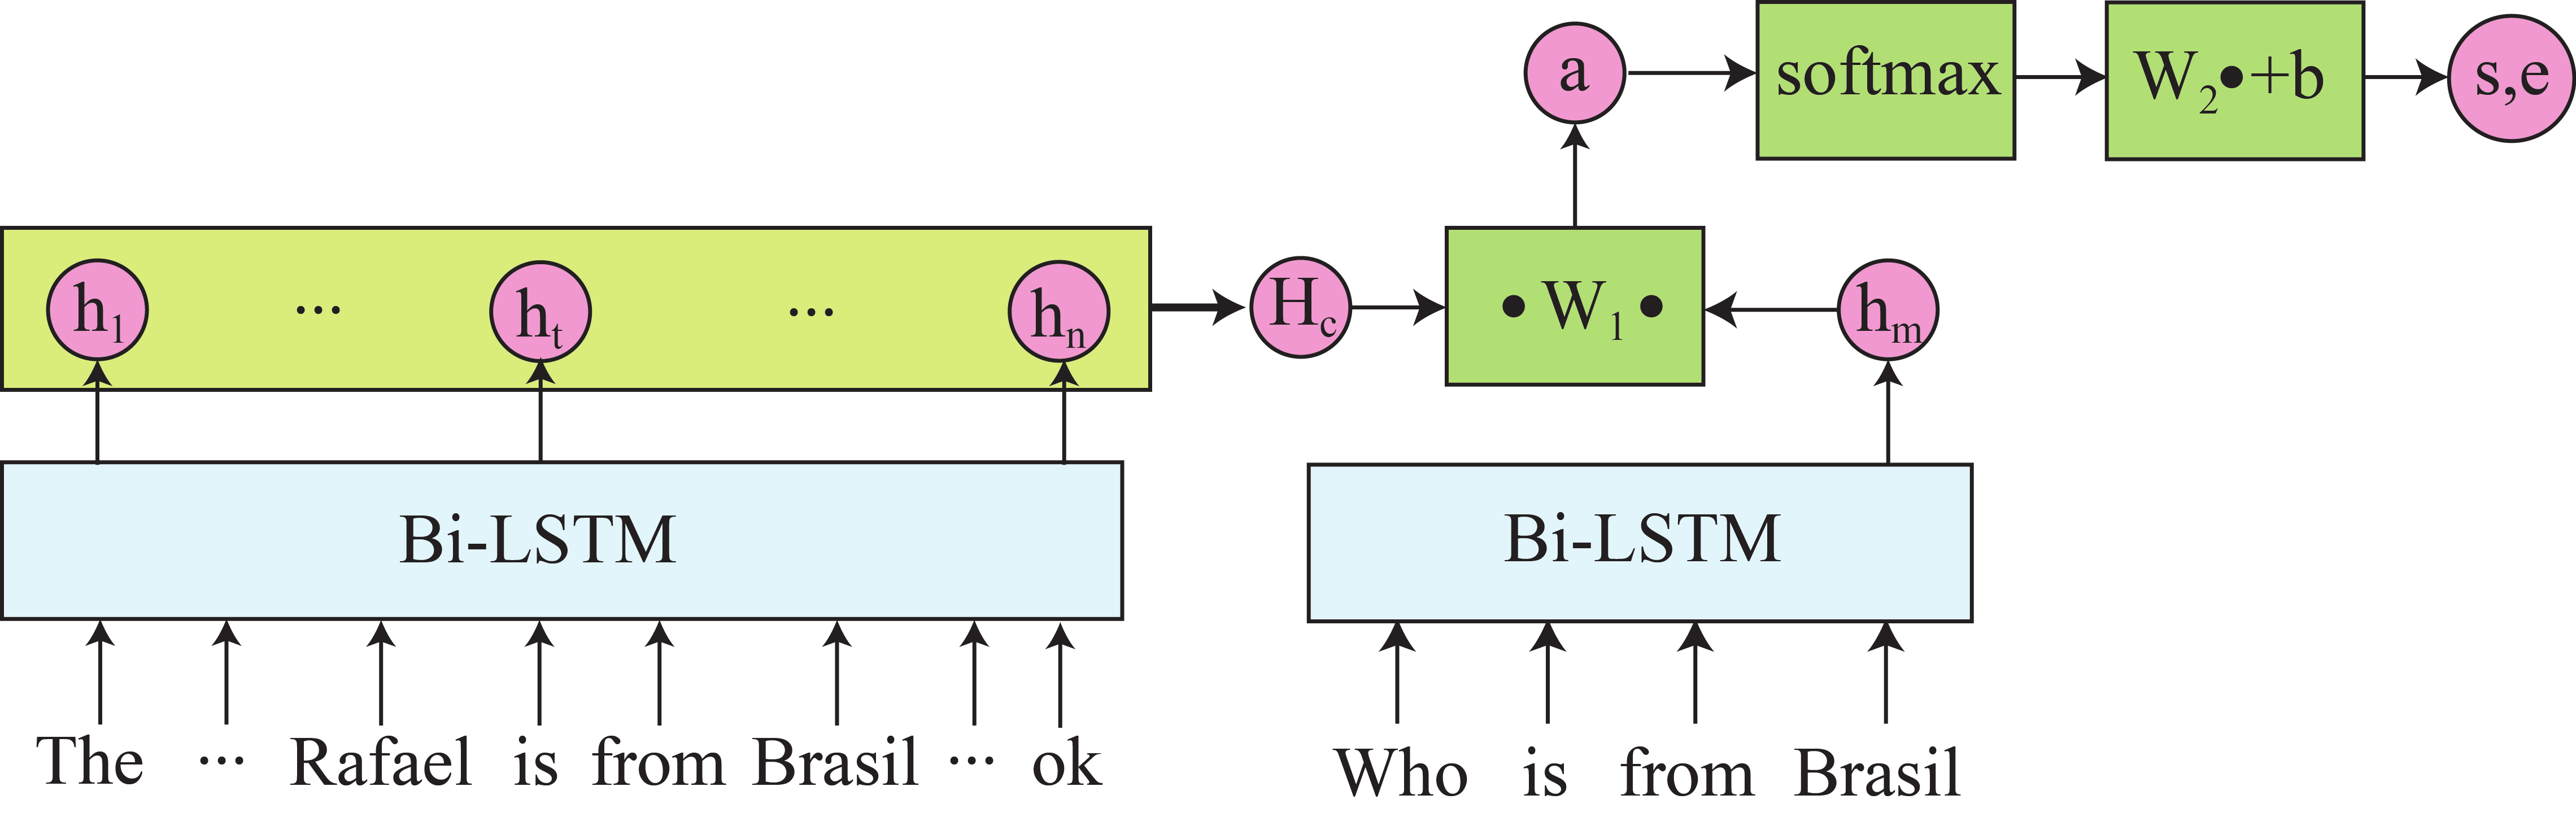
\includegraphics[width=\linewidth]{reader.png}
  \caption{ Attentive reader neural network }
  \label{fig:reader}
\end{figure}

This can be viewed as a generalization of the application of memory networks to question answering. This model employs an attention mechanism at the sentence level where each sentence is represented by a bag of embeddings. The attentive reader employs a fine grained token level attention mechanism where the tokens are embedded given their entire future and past context with in the story.

\section{DataSet}
\label{data_set}

The WIKI READING task requires to predict textual values from the open knowledge base Wikidata given text from the corresponding articles on
Wikipedia. Example instances are shown
in Table 1, illustrating the variety of subject mat-
ter and sub-tasks. The dataset contains 18.58M in-
stances across 884 sub-tasks, split roughly evenly
between classification and extraction
 
\begin{table}[h!]
\begin{tabular}{ |p{2cm}|p{2cm}|p{2cm}|p{2cm}|p{2cm}|  }
 \hline
 \multicolumn{1}{|c|}{} &
 \multicolumn{2}{|c|}{Categorization} &
 \multicolumn{2}{|c|}{Extraction} \\
 \hline
 Document & Folkart Towers are twin  skyscrapers  in  the Bayrakli  district  of  the Turkish   city   of   Izmir. Reaching    a    structural height of 200 m (656 ft) above ground level, they are the tallest... &Angeles   blancos   is   a Mexican telenovela produced   by   Carlos   Sotomayor  for  Televisa  in
1990.Jacqueline  Andere,Rogelio   Guerra and   Alfonso   Iturralde star as the main... &Canada is a country in  the  northern  part  of North  America.   Its  ten
provinces and three territories  extend  from  the
Atlantic to  the Pacific and  northward  into  the
Arctic Ocean, . . .&Breaking Bad is an American  crime  drama television  series  created and  produced  by  Vince Gilligan.The show originally  aired  on  the
AMC  network  for  five seasons,  from January 20, 2008, to . . .\\
 \hline
 Property   & country    &original language of work&   located  next  to  body  of water& start time\\
 \hline
 Answer &   Turkey  & Spanish &Atlantic  Ocean,   Arctic Ocean, Pacific Ocean& 20 January 2008\\
 \hline
\end{tabular}

\caption{Examples instances from WIKI READING. The task is to predict the answer given the document and property. Answer tokens that can be extracted are shown in bold, the remaining instances require classification or another form of inference.}
\label{table:1}
\end{table}

The  dataset  contains  4.7M  unique  Wikipedia  ar-
ticles, meaning that roughly 80 percent of the English language  Wikipedia  is  represented.   Multiple  in-
stances can share the same document, with a mean
of  5.31  instances  per  article  (median: 4,max:879).The  most  common  categories  of  documents  are
human,taxon,film,album,  and human settlement, making up 48.8 percent of the documents and 9.1 percent of the instances.  The mean and median document lengths are 489.2 and 203 words.

\section{Approach}
\label{approach}

Recently, neural network architectures for QA have  been  shown  to  meet  or  exceed  the  performance of traditional methods. The  move  to  deep  neural
networks  also  allows  for  new  ways  of  combin-
ing the property and document, inspired by recent
research in the field of question answering (with the  property  serving  as  a  question).   In  memory network models,  the  question  could  be
used to compute a form of attention over the document, to effectively focus the model on the most predictive words or phrases (Sukhbaatar et al.,  2015;  Hermann et al.,  2015). As this is currently an ongoing field of research,we have implemented them both to compare them on common grounds. We  now  describe  these  methods and introduce some adjustments to tackle the data set size.

\paragraph{Baseline LSTM}

This model is a simplified version of the Deep LSTM Reader proposed by Hermann  et  al. (2015). In  this  model,  an  LSTM reads  the property and document sequences word-by-word and the final state is used as the joint representation.  This is the simplest model that respects the order of the words in the document. In our implementation we use a single layer instead of two and a larger hidden size.

\paragraph{Memory Networks}

Our implementation closely follows  the  End-to-End  Memory Network  proposed  in  Sukhbaatar  et  al.  (2015). This  model maps   a   property p
and a list of sentences $x_1 ,...,x_n$ to a joint representation y by attending  over  sentences  in  the  document  as  follows:
The input encoder I converts a sequence of words
$x_i= (x_{i1},...,x_{iL_i})$ into a vector using an embedding matrix (equation 6), where $L_i$ is the length of sentence i.The property is encoded with the embedding matrix U (eqn. 7). Each sentence is encoded into two vectors, a memory vector (eqn. 7) and an output vector (eqn. 9), with embedding matrices M and C, respectively. The property encoding is used to compute a normalized attention vector over the memories (eqn. 10). The joint representation is the sum of the output vectors weighted by this attention
\begin{equation}
I(x_i,W) = \sum_j W x_{ij}
\end{equation}
\begin{equation}
m_i = I(x_i,M)
\end{equation}
\begin{equation}
c_i = I(x_i,C)
\end{equation}
\begin{equation}
p_i = Softmax(q^T m_i)
\end{equation}
\begin{equation}
y = u + \sum_i p_ic_i
\end{equation}

\paragraph{Attentive Reader}

This  model,  also  presented in Hermann et al. (2015), uses an attention mechanism  to  better  focus  on  the  relevant  part  of  the document for a given property.   Specifically,  Attentive Reader first generates a representation u of the property using the final state of an LSTM while a second LSTM is used to read the document and generate a representation $z_t$
for each word.  Then,conditioned on the property encoding u, a normalized attention is computed over the document to produce a weighted average of the word representations $z_t$, which is then used to generate the joint representation y. More precisely:

\begin{equation}
m_t = \tanh(W_1 concat(z_t,u))
\end{equation}
\begin{equation}
\alpha_t = \exp(v^T m_t)
\end{equation}
\begin{equation}
r = \sum_t \frac{\alpha_t}{\sum_i \alpha_i} z_t
\end{equation}
\begin{equation}
y = \tanh(W_2 concat(r,u))
\end{equation}

\section{Training}
\label{Training}
We used keras as the deep learning framework on top of tensorflow. The hardware we used is the NVIDIA TITAN x GPU that has 12 GB of memory. 

\begin{table}[h!]
\centering
\begin{tabular}{ |c|c|c|c|c| }
\hline
Method & Embedding Dimension & Vocab Size & Batch Size &Learnable Parameters\\
\hline 
 Baseline LSTM & 64 & 200K & 100 & 38M \\ 
 \hline
 MNN & 300 & 200k & 1000 & 91M\\  
 \hline
 ARNN & 128 & 200K & 500 & 46M \\
 \hline
\end{tabular}
\caption{Training Details}
\end{table}

Pruning: We weren't able to successfully train the model against some story sizes, being the entire wikipedia pages. So we pruned the document into manageable chunks by computing the similarity between the sentences and question and picking the top k. Clearly this isn't an ideal way, but we weren't able to investigate the model with some certainity with vocab size greater than this.

Evaluation: We evaluated all three methods on randomly sampled batches from separate test set using a single scoring framework.  An answer  is  correct  when  there  is  an  exact  string match between the predicted answer and the gold answer. However, some answers are composed from a set of values. To handle this, we define the Mean F1 score as follows:  For each instance, we compute the F1-score (harmonic mean
of precision and recall) as a measure of the degree
of overlap between the predicted answer set and
the gold set for a given instance. The resulting per-
instance F1 scores are then averaged to produce a
single dataset-level score.   This allows a method
to obtain partial credit for answers.

Some of the date related question types are clearly hard no matter which model we use. It seems the number
of supporting facts involved, the complexity of the
relation itself, and the length of the context makes it hard for the models to reason about.

\section*{GitHub}

\href{https://github.com/Ashwinasokan/LatentlyDeepLearningCertificate/tree/master/SukhbaatarSzlamWestonEtAl2015}{Project Repository}

\section*{Results}

\begin{table}[h!]
\centering
\begin{tabular}{ |c|c|c|c| }
\hline
Question Type & Baseline & MNN & ARNN \\
\hline 
 "country" & 0.14 & 0.46 & 0.38 \\ 
 \hline
 "occupation & 0.19 & 0.37 & 0.35\\  
 \hline
 "genre" & 0.17 & 0.32 & 0.31 \\
 \hline
 "sport" & 0.11 & 0.41 & 0.43\\
 \hline
 "date" & 0.08 & 0.11 & 0.07\\
 \hline
\end{tabular}
\caption{Accuracy on hold out data}
\end{table}

\begin{figure}[h]
  \centering
  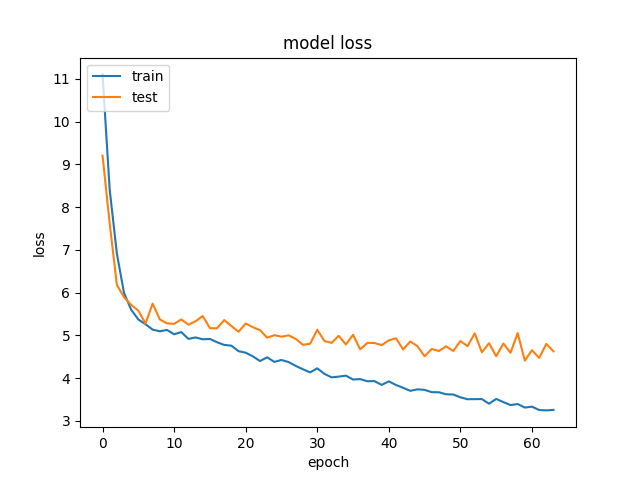
\includegraphics[scale=0.4]{loss.png}
  \caption{ Loss (MNN) }
  \label{fig:reader}
\end{figure}
\begin{figure}[h]
  \centering
  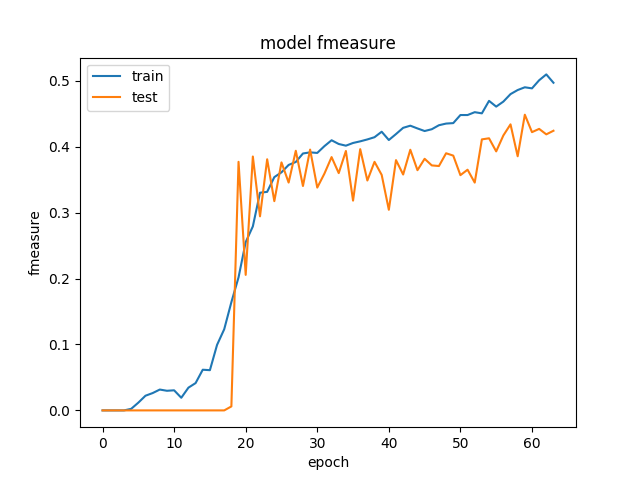
\includegraphics[scale=0.4]{f1.png}
  \caption{ F1 (MNN)}
  \label{fig:reader}
\end{figure}

\section*{Conclusion and Future Work}

In this project, we tried to evaluate the memory based neural models for the task of question answering from raw wikipedia pages. We started with a naive LSTM, based on the similarity of the question and input facts. The accuracy of the baseline is below .2 for all categories of the question. Then our model of choices MNN's and ARNN's did much better than the naive LSTM model in relatively better training time. We haven't tried multi layers in both the models, particularly MNN's. 

We have pruned sentences to contain data set with in the available memory footprint, which turned out to be the bottleneck, rather training a component separately to spot the relevant part of the story based on supervision seems promising lead. Still the training of the model on complete data set is possible if we could parallelize it. We haven't investigated much on that. Our best model was able to achieve 0.43 accuracy on the hold out set. At the moment, the models are traned separately based on question type, generalising it would be another challenge as well.


\section*{References}
\medskip

\small

[1] Daniel Hewlett.,\ Alexandre Lacoste.,\  Llion Jones.,\ Illia Polosukhin., \& Andrew Fandrianto\ (2016) WikiReading: A Novel Large-scale Language Understanding Task over Wikipedia, {\it Proceedings of the 54th Annual Meeting of the Association for Computational Linguistics 7}, pp.\ 1535-1545.

[2] Jason Weston.,\ Sumit Chopra.\& Antoine Bordes (2014) Memory Networks.

[3] Antoine Bordes, Nicolas Usunier, Sumit Chopra, \&  Jason Weston.\ (2015) Large-scale Simple Question Answering with Memory Networks.

[4] Sainbayar Sukhbaatar, Arthur Szlam, Jason Weston, \&  Et Al.\ (2015) End-To-End Memory Networks.

[5] Karl Moritz Hermann, Tomas Kocisky, Edward Grefenstette, \&  Et Al.\ (2015) Teaching Machines to Read and Comprehend.

[6] Ankit Kumar, Ozan Irsoy, Peter Ondruska, \&  Et Al.\ (2016) Ask Me Anything: Dynamic Memory Networks for Natural Language Processing, {\it Proceedings of The 33rd International Conference on Machine Learning} , PMLR 48:1378-1387.

[7] Matt J. Kusner, Yu Sun, Nicholas I. Kolkin, \&   	Kilian Q. Weinberger\ (2015) From word embeddings to document distances, {\it Proceeding
ICML'15 Proceedings of the 32nd International Conference on International Conference on Machine Learning} , Volume 37 Pages 957-966.

[8] Matthew Richardson, Christopher J.C. Burges, \&   	Erin Renshaw\ (2013) MCTest: A Challenge Dataset for the Open-Domain Machine Comprehension of Text, {\it Proceedings of the 2013 Conference on Emprical Methods in Natural Language Processing (EMNLP 2013) }

[9] Jason Weston, Antoine Bordes, \&   	Et Al\ (2015) Towards AI-Complete Question Answering: A Set of Prerequisite Toy Tasks, {\it Proceedings of the 2016 International Conference on Learning Representations (ICLR 2016) }

\end{document}
